%%!TEX encoding = UTF-8 Unicode

% According to UA rules, font size should range from 10 to 12pt.
\documentclass[11pt,a4paper,openright,final,twoside,onecolumn]{memoir}

\listfiles
\fixpdflayout

\usepackage[utf8]{inputenc}

% Computer Modern Typewritter (For bold ttfamily in listings)
\usepackage{lmodern}
% OR... Bera Mono
%\usepackage[scaled]{beramono} % TTT Font
%\usepackage{anyfontsize} % As the name says...

\usepackage[T1]{fontenc}

% For Overleaf support
\usepackage{ifthen}
\def\useoverleaf{1}  % change to non-zero (for instance, 1) to enable it

\makeatletter
\newcommand{\makecoverfile}[0]{%
  \immediate\write18{latexmk -pdf cover.tex}%
}
\makeatother

%For PDF merging
\usepackage{pdfpages}

%SET DPI to 300
\pdfpxdimen=\dimexpr 1in/300\relax

\usepackage{morewrites} % Allow the use of a larger number of packages

%For English and Portuguese languages
%Portuguese will be the default.
%Use \setdefaultlanguage to change it
\usepackage{csquotes}
\usepackage[english,portuguese]{babel}

% For custom date format
\usepackage{datetime}
\newdateformat{thesisdate}{\monthname[\THEMONTH] \THEYEAR} % Month Year

\usepackage{microtype} % Make pdf look better


% Uncomment to enable floats on facing pages
%\usepackage{dpfloat}

%Side by side figures
% Eg. Fig 1a, Fig 1b
\usepackage[hang,small,bf]{caption}
%\let\tion\undefined
%\let\subfloat\undefined
\usepackage{subcaption}

%\RequirePackage{textcase}

% Dropped Caps
%\usepackage{lettrine}


% Configure Hyperlink color
%\usepackage[breaklinks=true,colorlinks=false,linkcolor=blue]{hyperref}
% Or use the default
\usepackage{hyperref}

%Optional: Redefine section names
%\def\sectionautorefname{Section}
%\def\chapterautorefname{Chapter}
%\def\figureautorefname{Figure}
%\def\listingautorefname{Listing}
%\def\tableautorefname{Table}

%For PDF Comments
\usepackage{comment}
\usepackage{pdfcomment}
\usepackage{bookmark} % New Bookmarks

%For Multiple columns in Glossary
\usepackage{multicol}

%Math symbols
\usepackage{amsmath}
\usepackage{amssymb}

%Graphics
\usepackage{graphicx}

%Colors
\usepackage{xcolor}

%Euro symbol
\usepackage{eurosym}

% Code boxes
\ifthenelse{\equal{\useoverleaf}{0}}
{\usepackage[outputdir=build]{minted}}
{\usepackage{minted}}%

\renewcommand\listingscaption{Código}
\fvset{fontsize=\footnotesize} % Make Code blocks smaller than text

%Biber using IEEE style for proper UTF-8 support
\usepackage[backend=biber,style=ieee, sorting=none]{biblatex}
\bibliography{bib/Dissertation.bib, bib/references.bib, bib/rfc.bib}

%Use acronyms
\usepackage[printonlyused]{acronym} % For acronyms

% Enable chart support through pgf and tikz
\usepackage[version=0.96]{pgf}
\usepackage{tikz}
\usepackage{pgf-umlsd}
\usetikzlibrary{arrows,shadows,trees,shapes,snakes,automata,backgrounds,petri,mindmap} % for pgf-umlsd

%For Electric Circuits
\usepackage[detect-weight=true, binary-units=true]{siunitx}
\sisetup{load-configurations = binary}

\usepackage[american,cuteinductors,smartlabels]{circuitikz}

\usetikzlibrary{calc}
\ctikzset{bipoles/thickness=1}
\ctikzset{bipoles/length=0.8cm}
\ctikzset{bipoles/diode/height=.375}
\ctikzset{bipoles/diode/width=.3}
\ctikzset{tripoles/thyristor/height=.8}
\ctikzset{tripoles/thyristor/width=1}
\ctikzset{bipoles/vsourceam/height/.initial=.7}
\ctikzset{bipoles/vsourceam/width/.initial=.7}
\tikzstyle{every node}=[font=\small]
\tikzstyle{every path}=[line width=0.8pt,line cap=round,line join=round]

% For inline TT text (e.g. code snippets)
\usepackage{verbatim}

 %Frames around figures and allow force placement
\usepackage{float}

%Configure Float style
%\floatstyle{boxed}
%\restylefloat{table}
%\restylefloat{figure}
%\restylefloat{lstlisting}

%For test purposes
\usepackage{lipsum}

%Keep floats inside section!
\usepackage[section]{placeins}
\let \oldsubsubsection \subsubsection
\renewcommand{\subsubsection}[2][]{
  \FloatBarrier
  \oldsubsubsection#1{#2}
}
\let \oldsubsection \subsection
\renewcommand{\subsection}[2][]{
  \FloatBarrier
  \oldsubsection#1{#2}
}
\let \oldsection \section
\renewcommand{\section}[2][]{
  \FloatBarrier
  \oldsection#1{#2}
}
\let \oldchapter \chapter
\renewcommand{\chapter}[2][]{
  \FloatBarrier
  \oldchapter#1{#2}
}


%%%% Use the built-in division styling
\headstyles{memman}

%%% ToC down to subsections
\settocdepth{subsection}

%%% Numbering down to subsections as well
\setsecnumdepth{subsection}

%%%% extra index for first lines
\makeindex[lines]

%Margins for University of Aveiro Thesis
\setlrmarginsandblock{3cm}{2.5cm}{*}
\setulmarginsandblock{3cm}{3cm}{*}
\checkandfixthelayout

%Or custom spacing
%\addtolength{\parskip}{0.5\baselineskip}
\linespread{1.5}

\begin{document}
\ifthenelse{\equal{\useoverleaf}{0}}{}{\makecoverfile{}}%
\includepdf[pages=-]{cover.pdf}

%
%Front matter

%Custom Chapter style named thesis
\makechapterstyle{thesis}{% Based on ell
  \chapterstyle{default}
  \renewcommand*{\chapnumfont}{\normalfont\sffamily}
  \renewcommand*{\chaptitlefont}{\normalfont\Huge\sffamily}
  \settowidth{\chapindent}{\chapnumfont 111}
  \renewcommand*{\chapterheadstart}{\begingroup
    \vspace*{\beforechapskip}%
    \begin{adjustwidth}{}{-\chapindent}%
    \hrulefill
    \smash{\rule{0.4pt}{15mm}}
    \end{adjustwidth}\endgroup}
  \renewcommand*{\printchaptername}{}
  \renewcommand*{\chapternamenum}{}
  \renewcommand*{\printchapternum}{%
    \begin{adjustwidth}{}{-\chapindent}
    \hfill
    \raisebox{10mm}[0pt][0pt]{\fontsize{30}{25}\selectfont\chapnumfont \thechapter}%
                              \hspace*{1em}
    \end{adjustwidth}\vspace*{-3.0\onelineskip}}
  \renewcommand*{\printchaptertitle}[1]{%
    \vskip\onelineskip
    \raggedleft {\chaptitlefont ##1}\par\nobreak\vskip 4\onelineskip}}


%Select chapter style from existing or select custom
%\chapterstyle{thesis} % Others: dowding, demo2, dash, chappell, brotherton, bianchi, ger, madsen, tatcher, veelo,indexes)
% thesis can also be used as defined previously
%

%If you feel adventurous you can also define all aspects of your theme
%Use either this input or the chapterstyle before
%% Rules
\newcommand{\thinRule}{\rule{\textwidth}{0.25pt}}

% Customize heading appearances
% Define styles
\newcommand{\partSize}{\Huge}
\newcommand{\partStyle}{\lsstyle\scshape}
\newcommand{\chapterSize}{\Huge}
\newcommand{\chapterStyle}{\lsstyle\scshape}
\newcommand{\chapterAfter}{}
\newcommand{\sectionSize}{\Large}
\newcommand{\sectionStyle}{\scshape\MakeTextLowercase}
\newcommand{\subsectionSize}{\large}
\newcommand{\subsectionStyle}{\scshape\MakeTextLowercase}
\newcommand{\subsubsectionSize}{\large}
\newcommand{\subsubsectionStyle}{\scshape\MakeTextLowercase}
\newlength{\partNumSizePt}
\setlength{\partNumSizePt}{60pt}
\newlength{\chapterNumSizePt}
\setlength{\chapterNumSizePt}{60pt}
\newcommand{\partNumSize}{%
  \fontsize{\partNumSizePt}{1.2\partNumSizePt}\selectfont%
}
\newcommand{\partNumStyle}{\partChapterNumColor}
\newcommand{\chapterNumSize}{%
  \fontsize{\chapterNumSizePt}{1.2\chapterNumSizePt}\selectfont%
}
\newcommand{\chapterNumStyle}{\partChapterNumColor}

% Customize parts
\renewcommand{\partnamefont}{\partSize\partStyle}
\renewcommand{\partnumfont}{\partNumSize\partNumStyle}
\renewcommand{\printpartname}{}
\renewcommand{\printparttitle}[1]{%
  \normalfont\normalcolor\partnamefont #1
}

% Customize chapters
\makeatletter
\setlength{\beforechapskip}{30pt}
\renewcommand*{\chapterheadstart}{\vspace*{\beforechapskip}}
\setlength{\afterchapskip}{3ex}
\setlength{\midchapskip}{3ex}
\renewcommand*{\chapnamefont}{%
  \Large\flushright\chapterStyle\partChapterNumColor%
}
\renewcommand*{\chapnumfont}{\chapterNumSize\chapterNumStyle}
\renewcommand*{\chaptitlefont}{%
  \normalfont\flushleft\normalcolor\chapterSize\chapterStyle%
}
\renewcommand*{\printchaptername}{%
  \chapnamefont\MakeTextLowercase{\@chapapp}%
}
\renewcommand*{\chapternamenum}{\quad}
\renewcommand*{\printchapternum}{%
%  \chapnumfont\textls[-75]{\classicstylenums{\thechapter}}%
 \chapnumfont\textls[-75]{\thechapter}%

}
\renewcommand*{\printchaptertitle}[1]{%
  \chaptitlefont #1
  \chapterAfter
}
\makeatother
% Customize sections and subsections
\setsecnumformat{\csname my#1\endcsname\quad}
\setsecheadstyle{\sectionSize\sectionStyle}
\newcommand{\mysection}{{\thesection}}
\setlength{\beforesecskip}{3em}


\setsubsecheadstyle{\subsectionSize\subsectionStyle}
\newcommand{\mysubsection}{{\normalfont\subsectionSize\thesubsection}}
\setlength{\beforesubsecskip}{3em}

\setsubsubsecheadstyle{\subsubsectionSize\subsubsectionStyle}
\newcommand{\mysubsubsection}{{\normalfont\subsubsectionSize\thesubsubsection}}
\setlength{\beforesubsubsecskip}{2em}

% Customize "Table of ..." appearance
% Customize headings
\newcommand{\renewPrintXTitle}[1]{%
  \renewcommand{#1}[1]{%
    \printchaptertitle{##1}%
  }%
}
\renewPrintXTitle{\printtoctitle}
\renewPrintXTitle{\printlottitle}
\renewPrintXTitle{\printloftitle}

% Customize ToC headings
\renewcommand{\cftpartfont}{\partChapterNumColor\partStyle}
\renewcommand{\cftchapterfont}{\chapterStyle}
\renewcommand{\cftsectionfont}{}
\renewcommand{\cftsubsectionfont}{}
\renewcommand{\cftfigurefont}{}
\renewcommand{\cfttablefont}{}
\newcommand{\cftlstlistingfont}{}

% Increase number width
\newlength{\cftNumWidthIncrease}
\setlength{\cftNumWidthIncrease}{0.25em}
\addtolength{\cftpartnumwidth}{\cftNumWidthIncrease}
\addtolength{\cftchapternumwidth}{\cftNumWidthIncrease}
\addtolength{\cftsectionindent}{\cftNumWidthIncrease}
\addtolength{\cftsubsectionindent}{\cftNumWidthIncrease}
% No leader dots
%\renewcommand*{\cftpartdotsep}{\cftnodots}
%\renewcommand*{\cftchapterdotsep}{\cftnodots}
%\renewcommand*{\cftsectiondotsep}{\cftnodots}
%\renewcommand*{\cftsubsectiondotsep}{\cftnodots}
%\renewcommand*{\cftfiguredotsep}{\cftnodots}
%\renewcommand*{\cfttabledotsep}{\cftnodots}
%\newcommand*{\cftlstlistingdotsep}{\cftnodots}
% Set page numbers immediately after entry text
\newcommand{\tocEntryPageSep}{\hspace{1em}}
\renewcommand{\cftpartleader}{\cftdotfill{\cftdotsep}}
%\renewcommand{\cftpartafterpnum}{\cftparfillskip}
%\renewcommand{\cftchapterleader}{\tocEntryPageSep}
\renewcommand{\cftchapterleader}{\cftdotfill{\cftdotsep}}
%\renewcommand{\cftchapterafterpnum}{\cftparfillskip}
\renewcommand{\cftsectionleader}{\cftdotfill{\cftdotsep}}
%\renewcommand{\cftsectionafterpnum}{\cftparfillskip}
\renewcommand{\cftsubsectionleader}{\cftdotfill{\cftdotsep}}
%\renewcommand{\cftsubsectionafterpnum}{\cftparfillskip}
\renewcommand{\cftfigureleader}{\cftdotfill{\cftdotsep}}
%\renewcommand{\cftfigureafterpnum}{\cftparfillskip}
\renewcommand{\cfttableleader}{\cftdotfill{\cftdotsep}}
%\renewcommand{\cfttableafterpnum}{\cftparfillskip}
\newcommand{\cftlstlistingleader}{\cftdotfill{\cftdotsep}}
%\newcommand{\cftlstlistingafterpnum}{\cftparfillskip}
% Customize page numbers
\newcommand{\tocPageStyle}{\tocPageColor}
\renewcommand{\cftpartpagefont}{\tocPageStyle}
\renewcommand{\cftchapterpagefont}{\tocPageStyle}
\renewcommand{\cftsectionpagefont}{\tocPageStyle}
\renewcommand{\cftsubsectionpagefont}{\tocPageStyle}
\renewcommand{\cftfigurepagefont}{\tocPageStyle}
\renewcommand{\cfttablepagefont}{\tocPageStyle}
\newcommand{\cftlstlistingpagefont}{\tocPageStyle}

% Abstract
% Remove indents around abstract text
\setlength{\absleftindent}{0pt}
\setlength{\absrightindent}{0pt}
% Change font size to conform with the rest of the document text
\renewcommand{\abstracttextfont}{\normalsize}

% Customize headers and footers including page numbers
\newcommand{\hfTextSize}{\footnotesize}
\newcommand{\headTextStyle}{\lsstyle\scshape\MakeTextLowercase}
\nouppercaseheads
\makeevenhead{headings}%
             {\hfTextSize\thepage}%
             {}%
             {\hfTextSize\headTextStyle\leftmark}
\makeevenhead{plain}%
             {\hfTextSize\thepage}%
             {}%
             {\hfTextSize\headTextStyle\leftmark}
\makeoddhead{headings}%
            {\hfTextSize\headTextStyle\rightmark}%
            {}%
            {\hfTextSize\thepage}
\makeoddhead{plain}%
            {\hfTextSize\headTextStyle\rightmark}%
            {}%
            {\hfTextSize\thepage}



% Customize captions
\newcommand{\captionSize}{\small}
\newcommand{\captionStyle}{\scshape}
\newcommand{\captionWidthRatio}{0.9}

\captionnamefont{\captionSize\captionStyle}
\captiontitlefont{\captionSize}
\captiondelim{ -- }
\captiontitlefinal{}
\changecaptionwidth
%\captionwidth{\captionWidthRatio\textwidth}

% Define colors
%\newcommand{\titleColor}{\color[rgb]{0.616, 0.0627, 0.176}}
\newcommand{\titleColor}{\color[rgb]{0,0,0}}

\newcommand{\partChapterNumColor}{\titleColor}
\newcommand{\dropCapColor}{\titleColor}
%\newcommand{\tocPageColor}{\color[rgb]{0.0980, 0.329, 0.651}}

\newcommand{\tocPageColor}{\color[rgb]{0, 0,0}}
\definecolor{shade0}{rgb}{1.0 , 1.0 , 1.0 }
\definecolor{shade1}{rgb}{0.9 , 0.9 , 0.9 }
\definecolor{shade2}{rgb}{0.8 , 0.8 , 0.8 }
\definecolor{shade3}{rgb}{0.65, 0.65, 0.65}
\definecolor{shade4}{rgb}{0.45, 0.45, 0.45}
\definecolor{shade5}{rgb}{0.0 , 0.0 , 0.0 }



\chapterstyle{veelo}
%Exclude sub figures from List of Figures
%\captionsetup[subfloat]{list=no}


% Texts
\newenvironment{introduction}
{%
  \begin{minipage}{\textwidth}%
   \itshape%
}
{%
  \end{minipage}%
  \par\addvspace{2\baselineskip plus 0.2\baselineskip minus 0.2\baselineskip}%
}


%Select Page style
\pagestyle{plain}

\frontmatter

\tightlists
\midsloppy
\raggedbottom

\setcounter{tocdepth}{2} %subsections are added to the TOC
\setcounter{secnumdepth}{4} %subsubsections are numbered


\cleardoublepage

%Table of contents
{\small\tableofcontents}
\cleardoublepage

%List of figures
{\small\listoffigures}


%List of tables
\cleardoublepage
{\small\listoftables}

%Print Glossary
{\small\chapter{Acronyms}

\footnotesize
\SingleSpacing

\begin{multicols}{2}
\begin{acronym}[AAAAAA]

    \acro{API}[API]{Application Programming Interface}
	\acro{ANN}[ANN]{Artificial Neural Network}
	\acro{CNN}[CNN]{Convolutional Neural Network}

    \acro{GPU}[GPU]{Graphics Processing Unit}
	\acro{CPU}[CPU]{Central Processing Unit}
	\acro{RAM}[RAM]{Random Access Memory}

    \acro{TP}[TP]{True Positive}
    \acro{TN}[TN]{True Negative}
    \acro{FP}[TN]{False Positive}
    \acro{FN}[TN]{False Negative}
    \acro{TPR}[TPR]{True Positive Rate}
    \acro{TNR}[TNR]{True Negative Rate}
    \acro{FPR}[FPR]{False Positive Rate}
    \acro{PPV}[PPV]{Positive Predictive Value}
    \acro{NPV}[NPV]{Negative Predictive Value}
    \acro{AUC}[AUC]{Area Under Curve}
    \acro{ROC}[ROC]{Receiver Operating Characteristic}

    \acro{IEETA}[IEETA]{Instituto de Engenharia Eletrónica e informáTica de Aveiro}
    \acro{LAR}[LAR]{Laboratory for Automation and Robotics}
    \acro{ISIC}[ISIC]{International Skin Imaging Collaboration}
    \acro{ILSVRC}[ILSVRC]{ImageNet Large Scale Visual Recognition Competition}
    
    \acro{HAM10000}[HAM10000]{Human Against Machine with 10000 images}
    \acro{BCN_20000}[BCN20000]{BCN20000 with 19424 images}
    \acro{MSK}[MSK]{MSK data from ISIC archive}

\end{acronym}
\end{multicols}

}

%
%Main document starts here
%
\mainmatter



% Start of Thesis text ----------------------------------------------------------
%Line spacing: 1.5 pt
\OnehalfSpacing



\chapter{Introdução}
\label{chapter:introduction}

\begin{introduction}
A sort description of the chapter.

A memorable quote can also be used.
\end{introduction}

\section{Background}
Skin cancer is the most common type of cancer, particularly, in the United States of America the incidence rates keep rising with currently 1 in 5 persons developing skin cancer until the age of 70 \cite{Foundation2019}. However, skin cancer represents a problem not only for America but also for the international health community in general. For example, in Europe, over 100000 people are diagnosed with melanoma and 22000 deaths annually occur due to this form of skin cancer \cite{Bray2018}.  Yet, one of the most remarkable facts about skin cancer is that when detected on late stages there is a 23\% chance of survival, but when detected early the 5 year survival rate rises to 99\% \cite{Foundation2019}. Therefore, the early detection of skin cancer is an absolute priority. \par
Skin cancer can be detected by dermatology professionals by simple visual examination of skin lesions. However, the difference between malignant and benign skin lesions can be negligible making it a difficult task even for trained medical experts. As such, a medical application which provides automated skin lesion diagnosis for decision support is an welcome addition to this field. \par
Initially, automated diagnosis of skin lesions was made based on predefined techniques well known by dermatology professionals such as the ABCDE rule (Asymmetry, Border, Color, Dermoscopic structure and Evolving), but often failed to either generalize to new cases or lacked the accuracy of a human. However, in more recent years, machine learning approaches into skin lesion diagnosis shows remarkable performance in comparison with the hand crafted algorithms, specially with deep learning methods\cite{Esteva2017}\cite{Haenssle2018}. 
\section{Objectives and Motivation}
A strong assumption can be made that if an accurate automated skin lesion diagnosis tool is used by dermatologists, then skin cancer cases will be detected earlier. Therefore, the main objective behind this dissertation is to improve the current work on automated skin lesion diagnosis by using deep learning techniques. This work will be part of a tool that has the intent of being used in a clinic context, so the priority is to its performance as much as possible. \par 
Finally, the aforementioned tool must be packaged within a eHealth application, in order to be easily accessed by medical professionals in a clinical environment. Such application must have the ability to potentially integrate other components useful for both dermatologists and patients while enabling easy communication between them. 




\chapter{State of the art}
\label{chapter:sota}

The following sections are structured as follows. Section 2.1 provides an exploratory look into eHealth/mHealth applications for skin lesion diagnosis. Section 2.2 gives an overview of deep learning applied into medical imaging. Finally, Section 2.3 reviews some of the current approaches towards skin lesion diagnosis systems using deep learning.


\section{Methods and materials}
The following sections are structured as follows. Section 3.1 provides an explanatory view into the most used image recognition neural network typology. Section 3.2 describes two of the most popular \ac{CNN} architectures. Section 3.3 explores the concept of repurposing pre-trained models from \ac{CNN} architectures trained on generic datasets. Section 3.4 explores problems related to training deep networks and some solutions. Finally, Section 3.5 explores state of the art frameworks for training and deploying deep networks.   
\subsection{Artificial Neural Networks}
Artificial Neural Networks (\ac{ANN}s) compose a category of machine learning algorithms that are inspired by biological neural networks. These structures are comprised by multiple layers, each composed by multiple neurons that can be interpreted as a function described by parameters.
Within a neuron, each input $x_i$ is multiplied by a learnable matrix of weights $w_i$, where each weight can be seen as the synaptic strength between two neurons. A second parameter is also taken into consideration called bias $b$ that is added to the element wise multiplication between the weights and inputs matrices.  With this two parameters a neuron will output a signal according to a activation function $f$ which introduces non-linearity. Mathematically speaking, the output of a neuron can be expressed as Equation \ref{eqs:neuron}.
\begin{equation}
    f(\sum_{i}^{n} x_i w_i + b)
    \label{eqs:neuron}
\end{equation}
Some activation functions that can be used are:
\begin{itemize}
    \item The sigmoid function $f(x) = (\frac{1}{1+exp^{-x}})$. Provides smooth gradient between 0 and 1 values, but suffers from computation issues (vanishing gradients problem).
    \item The tanh function $f(x) = (\frac{e^x - e^{-x}}{e^x + e^{-x}}) $. Like the sigmoid except that output values range from -1 to 1, meaning it's center is at 0.  
    \item The ReLU function $f(x) = max(0, x)$. A network with such neurons is able to overcome numerical computation issues (exploding and vanishing gradients, typically associated with activation functions like the signmoid function) which, in practice, allow faster convergence \cite{?}.
    \item The softmax function $f(x_i) = \frac{exp(x_i)}{\sum_{i}^{} exp(x_j)}$. It is typically used in the output layer for neural networks which classify inputs into multiple classes. It normalizes the outputs for each class between 0 and 1, and divides by their sum, giving the probability of the input value being in a specific class \cite{?}.
\end{itemize}

We can look at \ac{ANN}s as an iterative process that tries to optimize parameters in order to minimize a cost function. \par
\ac{ANN}s can approximate any function with just one layer but for more complex functions an increased hidden width may be required which cloud limit it's capability \cite{?}. Therefore, networks with many more layers and with an organization which allows them to create levels of abstraction are often used to solve more complex problems. We call such networks deep neural networks. \par
There are many different typologies of \ac{ANN}s. The most common has a fully connected structure between layers, where each neuron is connected to every other neuron in the previous layer. 

However, in image recognition such network architecture does not take into account the spatial structure of images. For example, it treats input pixels which are far apart and close together on exactly the same footing. \par
\begin{figure}[ht]
  \centering
    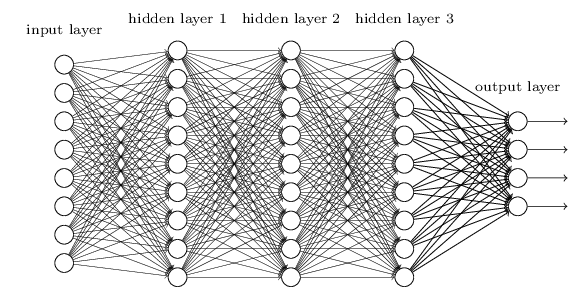
\includegraphics[scale=0.5, width=\linewidth]{figs/Deep_Learning.png}
  \caption{Artificial neural network \cite{vggnet}}
  \label{fig:fcnn}
\end{figure}
\subsection{Convolutional Neural Networks}
Instead, convolutional neural networks (\ac{CNN}) or some close variant are used in most neural networks for image recognition problems\cite{Nielsen2017a}. They still retain the core concepts of \ac{ANN}s, but add 3 different concepts which distinguish them from conventional \ac{ANN}s:
\begin{itemize}
\item Local receptive fields: In Figure \ref{fig:fcnn} inputs were depicted as a vertical line of neurons that were fully connected to the next hidden layer. However, for images inputs are pixel intensities in 2D space. Convolutional layers exploit this concept by only connecting neurons to a particular region of the input volume which ensures that the learnt filters activate strongly only in the presence of a spatially local input pattern. That region of the input is called local receptive field and is usually characterized by it's square size (5x5 for example) and it's stride length which can be 1 or more. Note that if we consider 5 x 5  local receptive field with stride 1 and a 28 x 28 input image then there will be 24 x 24  neurons in the hidden layer, because it can only move 23 neurons across.  
\item Shared weights: Weights and biases are shared across the hidden neurons so that convolutional networks become well adapted to translation variances in images. The shared weights are often said to define a kernel or filter, while to the map from the input layer to the hidden layer we call feature map, where a feature detected by a hidden neuron is some kind of input pattern that will cause the neuron to activate. To do image recognition we need multiple feature maps in order to recognize multiple features.
\item Pooling layers: These layers simplify the information in the output from the convolutional layer by removing unnecessary information, such as noise. A common pool layer is max pooling which provides a way to know if a given feature is found anywhere in a region of a image. For each feature map, it works by sliding a filter of size l x l with a specific stride S and computing the maximum value for the selected part of the input (illustrated in figure \ref{fig:maxpooling}). Overall this reduces the number of free parameters (while introducing no new parameters since max pooling is a fixed function of the input) and the memory footprint and computation in the network \cite{Nielsen2017a}.
\begin{figure}[ht]
  \centering
    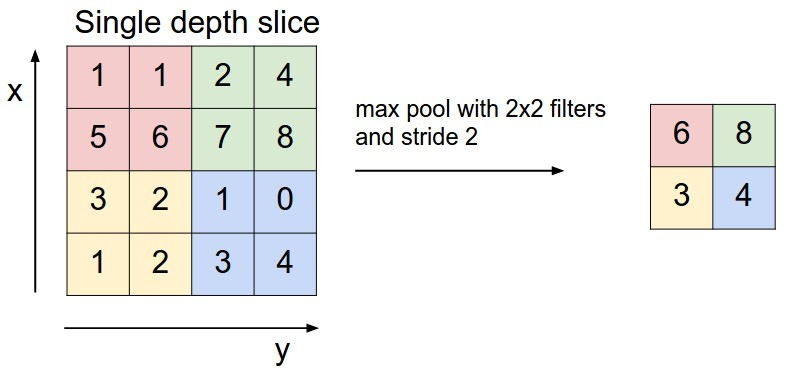
\includegraphics[width=0.5\linewidth]{figs/maxpooling.png}
  \caption{Max pooling with a 2 × 2 filter and stride S = 2 \cite{Nielsen2017a}}
  \label{fig:maxpooling}
\end{figure}
\end{itemize}
As a result of these 3 concepts the overall architecture of convolutional neural networks becomes quite different from fully connected neural networks but the same basic concepts still applies. Namely, the main objective is still to train the networks weights and biases in order for the network to have good perform classifying the inputs, It also still uses the same stochastic gradient descent and backpropagation algorithms. \par 
Illustrated in Figure \ref{fig:cnn}) is a convolutional neural network used to classify numbers from 28x28 images. It has  28 x 28 input neurons used to encode the pixel intensities, then is followed by a convolutional layer using a 5 x 5 local receptive field and 3 feature maps which results in 3 x 24 x 24 feature neurons. Next, a max-pooling layer is applied with 2 x 2 regions of stride 2 which results in 3 x 12 x 12 hidden feature neurons. Finally, the output layer has a fully connected structure (which is not fully connected in the figure for simplicity) with 10 neurons, because the objective of the network is to classify digits between 0 and 9 , meaning that it has 10 different classes to classify and therefore should have 10 different output neurons. \par
\begin{figure}[ht]
  \centering
    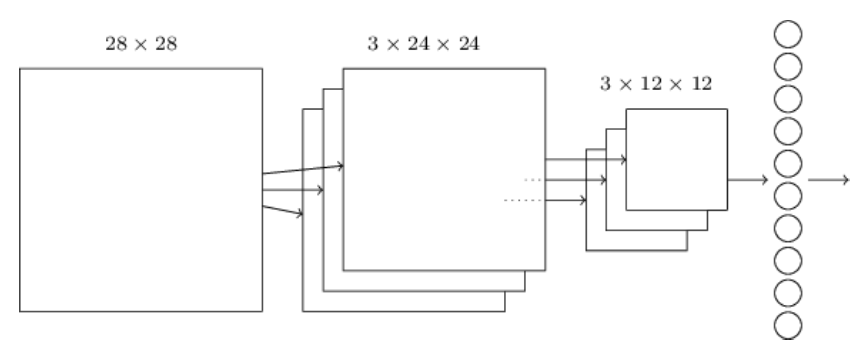
\includegraphics[width=0.5\linewidth]{figs/cnn.png}
  \caption{Convolutional neural network architecture used to classify digits from the MNIST dataset \cite{Nielsen2017a}}
  \label{fig:cnn}
\end{figure}
This represents a simple CNN architecture for a simple problem. However, even in this scenario we can already see that the number of learnable parameters escalates quickly in this type of networks. As such, it is crucial to develop highly efficient and effective architectures for more complex problems. 
\subsection{Convolutional neural network architectures}
Over the years several \ac{CNN} architectures have been developed and tested against state of the art benchmark challenges such as the \ac{ILSVRC} \cite{ilsvrc}. In 2012, Krizhevsky et al. \cite{alexnet} submited for the first time a \ac{CNN} architecture (AlexNet) which outperformed hand-crafted feature learning on the ImageNet. It contained 8 neural network layers, 5 convolutional and 3 fully-connected. This laid the foundation for traditional \ac{CNN}s: a convolutional layer followed by an activation function followed by a max pooling operation. \par
Following AlexNet main ideas, the VGGNet\cite{vggnet} was created and became quite popular by winning the 2014’s ILSVR. This architecture proved that representation depth is beneficial for the classification accuracy, by using the traditional convolutional network architecture but with increased depth along with smaller receptive fields. There are some public variations of this network, one of which having 16 weight layers (VGG16) displayed in Fig. 1. This architecture is composed by multiple sets of convolutional layers followed by pooling layers that build progressively more abstract features, and at the end a fully connected structure to convert the results of the convolution into a label.
\begin{figure}[ht]
  \centering
    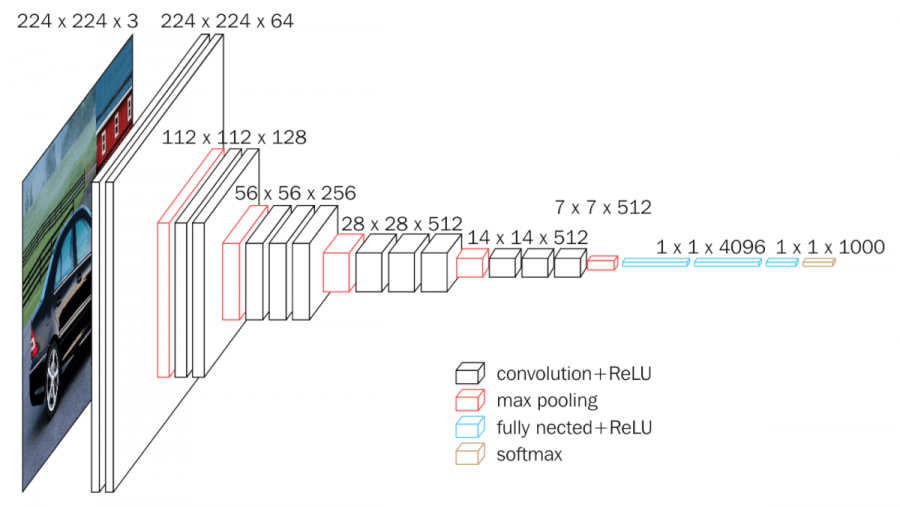
\includegraphics[scale=0.5, width=\linewidth]{figs/vgg16.png}
  \caption{Architecture of the VGG16 convolutional neural network \cite{vggnet}}
\end{figure}
\par
Until this point, both AlexNet and VGGNet use plain networks, which are networks that stack convolutional layers followed by fully connected layers and both approaches explore the idea of creating deeper networks in order to obtain better performance. However, at a certain point when the network becomes too deep, the problem of vanishing gradients starts to be prominent. The reason behind this problem is that on deep networks as the gradient is back-propagated to earlier layers, repeated multiplication may make the gradient infinitely small. Consequently, as the network becomes  deeper, its performance gets saturated or even starts degrading rapidly. \par
In 2015 a team of Microsoft researchers won the ILSVR, and later submitted a paper to the 2016's CVPR, in which they show that a 20 layer plain network performs better than a 56-layer plain network one due to the presence of the vanishing gradients problem on the deeper network. As such, they attempt to solve this problem with the introduction of a concept called skip connections seen in Fig. x. They hypothesize that letting the stacked layers fit a residual mapping is easier than letting them directly fit the desired underlaying mapping. \par
\begin{figure}[ht]
  \centering
    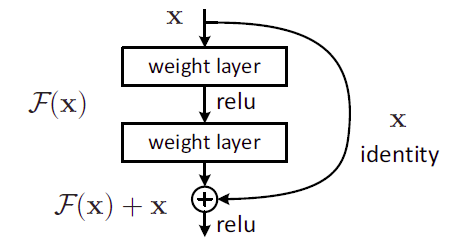
\includegraphics[width=0.5\linewidth]{figs/skip_connection.png}
  \caption{Building block of residual networks \cite{resnet}}
\end{figure}
\par
The fundamental idea behind skip connections is to learn a kind of residual mapping: 
\begin{equation}
    F(x)=H(x)-x
\end{equation}
The advantage of ResNets is that the gradient can flow directly through the identity function from later layers to earlier layers, which helps with the vanishing gradient problem. \par
Several ResNets are available with different depths. Some of the most popular variations have 50, 101 and 152 layers which had top 1 accuracy scores on the ImageNet dataset of 0.749, 0.764, 0.766, respectively. 
However, as Huang et al. pointed out, when the output of a layer l is combined with the identity function by summation, the information flow of the network may be compromised, meaning that some information might be lost in this process. Therefore, they extended the skip connection concept further in their work at \cite{densenet} with the introduction of a new type of neural network called Dense Convolutional Network (DenseNet). \par
Unlike ResNets, any layer has direct connections to all subsequent layers, and feature maps are combined with concatenation instead of summation. Authors argue that concatenating feature-maps learned by different layers further improves information flow efficiency and increases variation of subsequent layers. Consequently, the $l$th layer receives the feature-maps of all preceding layers, $ x_0, . . . , x_{l-1} $, as input:
\begin{equation}
    x_l = H_l([x_0, x_1, . . . , x_{l-1}])
\end{equation}
where $ [x_0, x_1, . . . , x_{l-1}] $ refers to the concatenation of the feature-maps produced in layers $ 0, . . . , l-1 $. Figure \ref{fig:densenet} illustrates the DenseNet schematics.

\begin{figure}[ht]
  \centering
    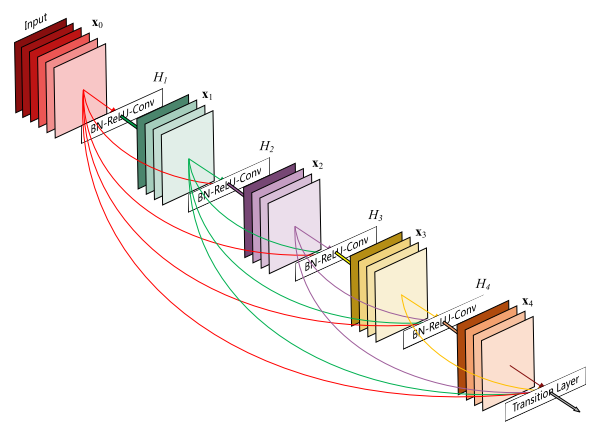
\includegraphics[width=0.5\linewidth]{figs/densenet.png}
  \caption{A block from DenseNet with five layers. Each layer combines all preceding feature maps through concatenation. \cite{densenet}}
  \label{fig:densenet}
\end{figure}

Similarly to ResNet, DenseNet provides different versions with different depths, with 121, 169 and 201 layers performing slightly better than ResNet on ImageNet with top-1 accuracies of 0.750, 0.762, 0.773.

So far, the presented architectures explore the idea of scaling up depth of the network in other to build progressively more abstract features, however, there are three dimensions in which one can scale a network  (illustrated in Figure \ref{fig:modelscaling}): 
\begin{itemize}
    \item Width scaling controls the width of each layer on the model (Figure \ref{fig:modelscaling} (b)). Wider networks tend to be able to capture more fine-grained features and are easier to train, but extremely wide, shallow networks tend to have difficulties in capturing higher level features \cite{efficientnet}.
    \item Depth scaling controls how many layers the model has. All the former presented models explore the idea of scaling up the network in order to capture richer and more abstract features. However, as we've seen problems emerge from creating deeper networks, specifically, vanishing gradients. Approaches like \cite{resnet} and \cite{densenet} attempt to solve this problem but performance gains diminishes as models become deeper. For example, ResNet-101 and ResNet-1000 have very similar accuracy \cite{resnet}.
    \item Resolution scaling corresponds to the increase of resolution of input images. The intuition behind this type of scaling is that the network can see more detail and therefore capture more fin-grained patterns. 
\end{itemize}
Tan et al. noted these three scaling dimentions are not independent. Rather, intuition tells us that for higher resolution input images, there should be a depth increase such that the larger receptive fields capture similar features that include more pixels in bigger images. It also tells us that we should increase the network width in order to capture more fine-grained pattterns, because the images have more information (more pixels). Following this ideas, they proposed a new family of models called EfficientNets \cite{efficientnet} which coordinates and balances different scaling dimentions together through the compound scaling method presented in equation \ref{eqs:efficientnetcompound}. \par
\begin{equation}
    \begin{split}
        \text{depth: } d = \alpha^\theta \\
        \text{width: } w = \beta^\theta \\
        \text{resolution: } r = \gamma^\theta \\
        \text{s.t. } \alpha\cdot\beta^2\cdot\gamma^2\approx2 \\
        \alpha \geq 1, \beta \geq 1, \gamma \geq 1
        \label{eqs:efficientnetcompound}
    \end{split}
\end{equation}

They created a baseline model EfficientNet-B0 and then scaled up the model in three dimentions following those constraints creating 7 other models (EfficientNet-B1 to EfficientNet-B7) which increasingly have more parameters and FLOPS, but also in theory should have increasingly better performance. The idea is to provide a family of models that can be adapted to one's needs, depending on the available compute capability.

\begin{figure}[ht]
  \centering
    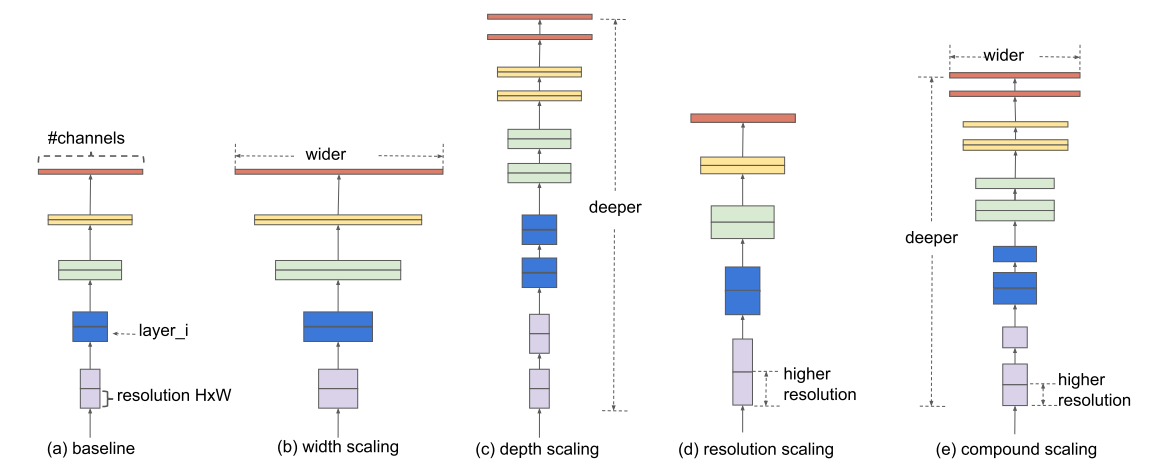
\includegraphics[scale=0.5, width=\linewidth]{figs/modelscaling.png}
  \caption{Model scaling methods. \cite{efficientnet}}
  \label{fig:modelscaling}
\end{figure}

Multiple pre trained models trained on ImageNet can be seen in Table \ref{tables:pretrainedmodels}, including the ones referenced so far. https://github.com/albanie/convnet-burden
https://keras.io/applications/

\begin{table}[h]
    \centering
    \begin{tabularx}{\textwidth}{|l|X|X|X|X|X|X|X|X|}
        \hline
        Model & Year & Size & Top-1 Accuracy & Top-5 Accuracy & Params & Depth & Input Size \\ \hline
        AlexNet & 2012 & 233 MB & ? & ? & $\approx$60M & 8 & 256x256 \\ \hline
    	VGG16 & 2014 & 528 MB & 0.713 & 0.901 & $\approx$138,4M & 23 & 224x224 \\ \hline
    	VGG19 & 2014 & 549 MB & 0.713 & 0.900 & $\approx$143,7M & 26 & 224x224 \\ \hline
    	ResNet50 & 2015 & 98 MB & 0.749 & 0.921 & $\approx$25,6M & - & 224x224 \\ \hline
    	ResNet101 & 2015 & 171 MB & 0.764 & 0.928 & $\approx$44,7M & - & 224x224 \\ \hline
    	ResNet152 & 2015 & 232 MB & 0.766 & 0.931 & $\approx$60,2M & - & 224x224 \\ \hline
    	ResNet50V2 & 2016 & 98 MB & 0.760 & 0.930 & $\approx$25,6M & - & 224x224 \\ \hline
    	ResNet101V2 & 2016 & 171 MB & 0.772 & 0.938 & $\approx$44,7M & - & 224x224 \\ \hline
    	ResNet152V2 & 2016 & 232 MB & 0.780 & 0.942 & $\approx$60,4M & - & 224x224 \\ \hline
        DenseNet121 & 2016 & 33 MB & 0.750 & 0.923 & $\approx$8,1M & 121 & 224x224 \\ \hline
    	DenseNet169 & 2016 & 57 MB & 0.762 & 0.932 & $\approx$14,3M & 169 & 224x224 \\ \hline
    	DenseNet201 & 2016 & 80 MB & 0.773 & 0.936 & $\approx$20,2M & 201 & 224x224 \\ \hline
    	InceptionV3 & 2015 & 92 MB & 0.779 & 0.937 & $\approx$23,9M & 159 & 299x299 \\ \hline
    	InceptionResNetV2 & 2016 & 215 MB & 0.803 & 0.953 & $\approx$55,9M & 572 & 299x299 \\ \hline
     	Xception & 2016 & 88 MB & 0.790 & 0.945 & $\approx$22,9M & 126 & 299x299 \\ \hline
    	EfficientNetB0 & 2019 & 5.3 MB & 0.773 & 0.935 & $\approx$5,3M & 201 & 224x224 \\ \hline
    	EfficientNetB1 & 2019 & 7.9 MB & 0.792 & 0.945 & $\approx$7,8M & 201 & 240x240 \\ \hline
    	EfficientNetB2 & 2019 & 9.2 MB & 0.803 & 0.950 & $\approx$9,2M & 201 & 260x260 \\ \hline
    	EfficientNetB3 & 2019 & 12.3 MB & 0.817 & 0.956 & $\approx$12M & 201 & 300x300 \\ \hline
    	EfficientNetB4 & 2019 & 19.5 MB & 0.830 & 0.963 & $\approx$19M & 201 & 380x380 \\ \hline
    	EfficientNetB5 & 2019 & 30.6 MB & 0.837 & 0.967 & $\approx$30M & 201 & 456x456 \\ \hline
    	EfficientNetB6 & 2019 & 43.3 MB & 0.842 & 0.968 & $\approx$43M & 201 & 456x456 \\ \hline
    	EfficientNetB7 & 2019 & 66.7 MB & 0.844 & 0.971 & $\approx$66M & 201 & 224x224 \\ \hline
    \end{tabularx}
    \caption{Pre-trained models comparison}
    \label{tables:pretrainedmodels}
\end{table} 

\subsection{Transfer learning}
Training deep neural networks from scratch is often a difficult process because it requires:
\begin{itemize}
\item large amounts of labelled data that closely resembles the field it tries to describe 
\item time to train which is largely dependent on the computational power available 
\item ability to reason about hyper parameters and follow heuristics in order to achieve a good model on the cross validation process
\end{itemize}
However, these requirements can be quite difficult to attain specially for small teams with limited monetary and human resources. Particularly in the medical imaging context, public datasets to train deep networks are rather scarce, mainly because of the nature of such data, that expose patients leading to a lack of privacy and anonymity. 
Even when one has a good dataset along with high computational power, the training process can take a long time, especially while debugging the network to determine a good model fit. \par
As such, transfer learning emerged as a way to solve this problem, by  relaxing the need for the aforementioned requirements. Transfer learning is a method of reusing a pre trained model's knowledge for another related task\cite{DipanjanSarkarRaghavBali2018}. In deep learning, using transfer learning means to carry the parameters from pre-trained models such as the architectures presented in Section 3.2 trained on a generic datasets such as ImageNet and using those to train another model with a different purpose.\par Transfer learning techniques are usually used to solve image classification problems \cite{Ly2019} because it leverages general knowledge from pre trained models towards specific purposed models. \par
In \ac{CNN}s, as inputs are passed along the network hidden layers closer to the input layer output generic features like shapes and curves, while hidden layers closer to the output layers build more abstract features such as a dog's face. In order to adapt the pre-trained models into a different domain, one must extract the parameters up to some layer from the pre-trained model while freezing (to not allow parameter updates while training) some or no portion of those layers. As layers near the input layer output generic features, their parameters are usually extracted and potentially frozen, while hidden layers near the output layer are usually not extracted and not frozen, because they output more abstract problem specific features. Figure \ref{fig:transferlearning} illustrates 3 different strategies to deal 
When repurposing the knowledge from a pre trained model one must first remove it's classifier, and replace it by a classifier that fits one's needs, while keeping the rest of the architecture (called convolutional base) intact. Figure \ref{fig:transferlearning} illustrates 3 different strategies to repurpose a pre-trained model:
\begin{itemize}
    \item Strategy 1: Fine tune the whole model. Often requires both more computational power, due to having more parameters to train, and more data to adapt the model to it's new purpose. 
    \item Strategy 2: Freeze part of the model while fine tuning the remaining layers. As previously mentioned lower layers identify problem independent features, while higher layers refer to problem dependent features. As such, one can chose up to which layer should the model be freezed depending on how much different his problem is compared to the original pre trained model problem. Some general advice can be given about this type of strategy. If the dataset to train the pre trained model is big enough and enough computational power is available the benefits of fine tuning more layers outweight the cons (namely more time to train the model). However, if one has a big enough dataset and low computational power, only fine tuning higher layers might be preferable. TODOOOOOOO  
    \item Strategy 3: Keep the convolutional base parameters and only train the classifier. Usually used in cases where the purpose of the pre-trained model is very similar to the problem that we are trying to solve, meaning that the datasets are similar. This is can be a especially good strategy if the available computational pwoer is low because the only parameters required to train are the classifier one's.
\end{itemize}

\begin{figure}[ht]
  \centering
    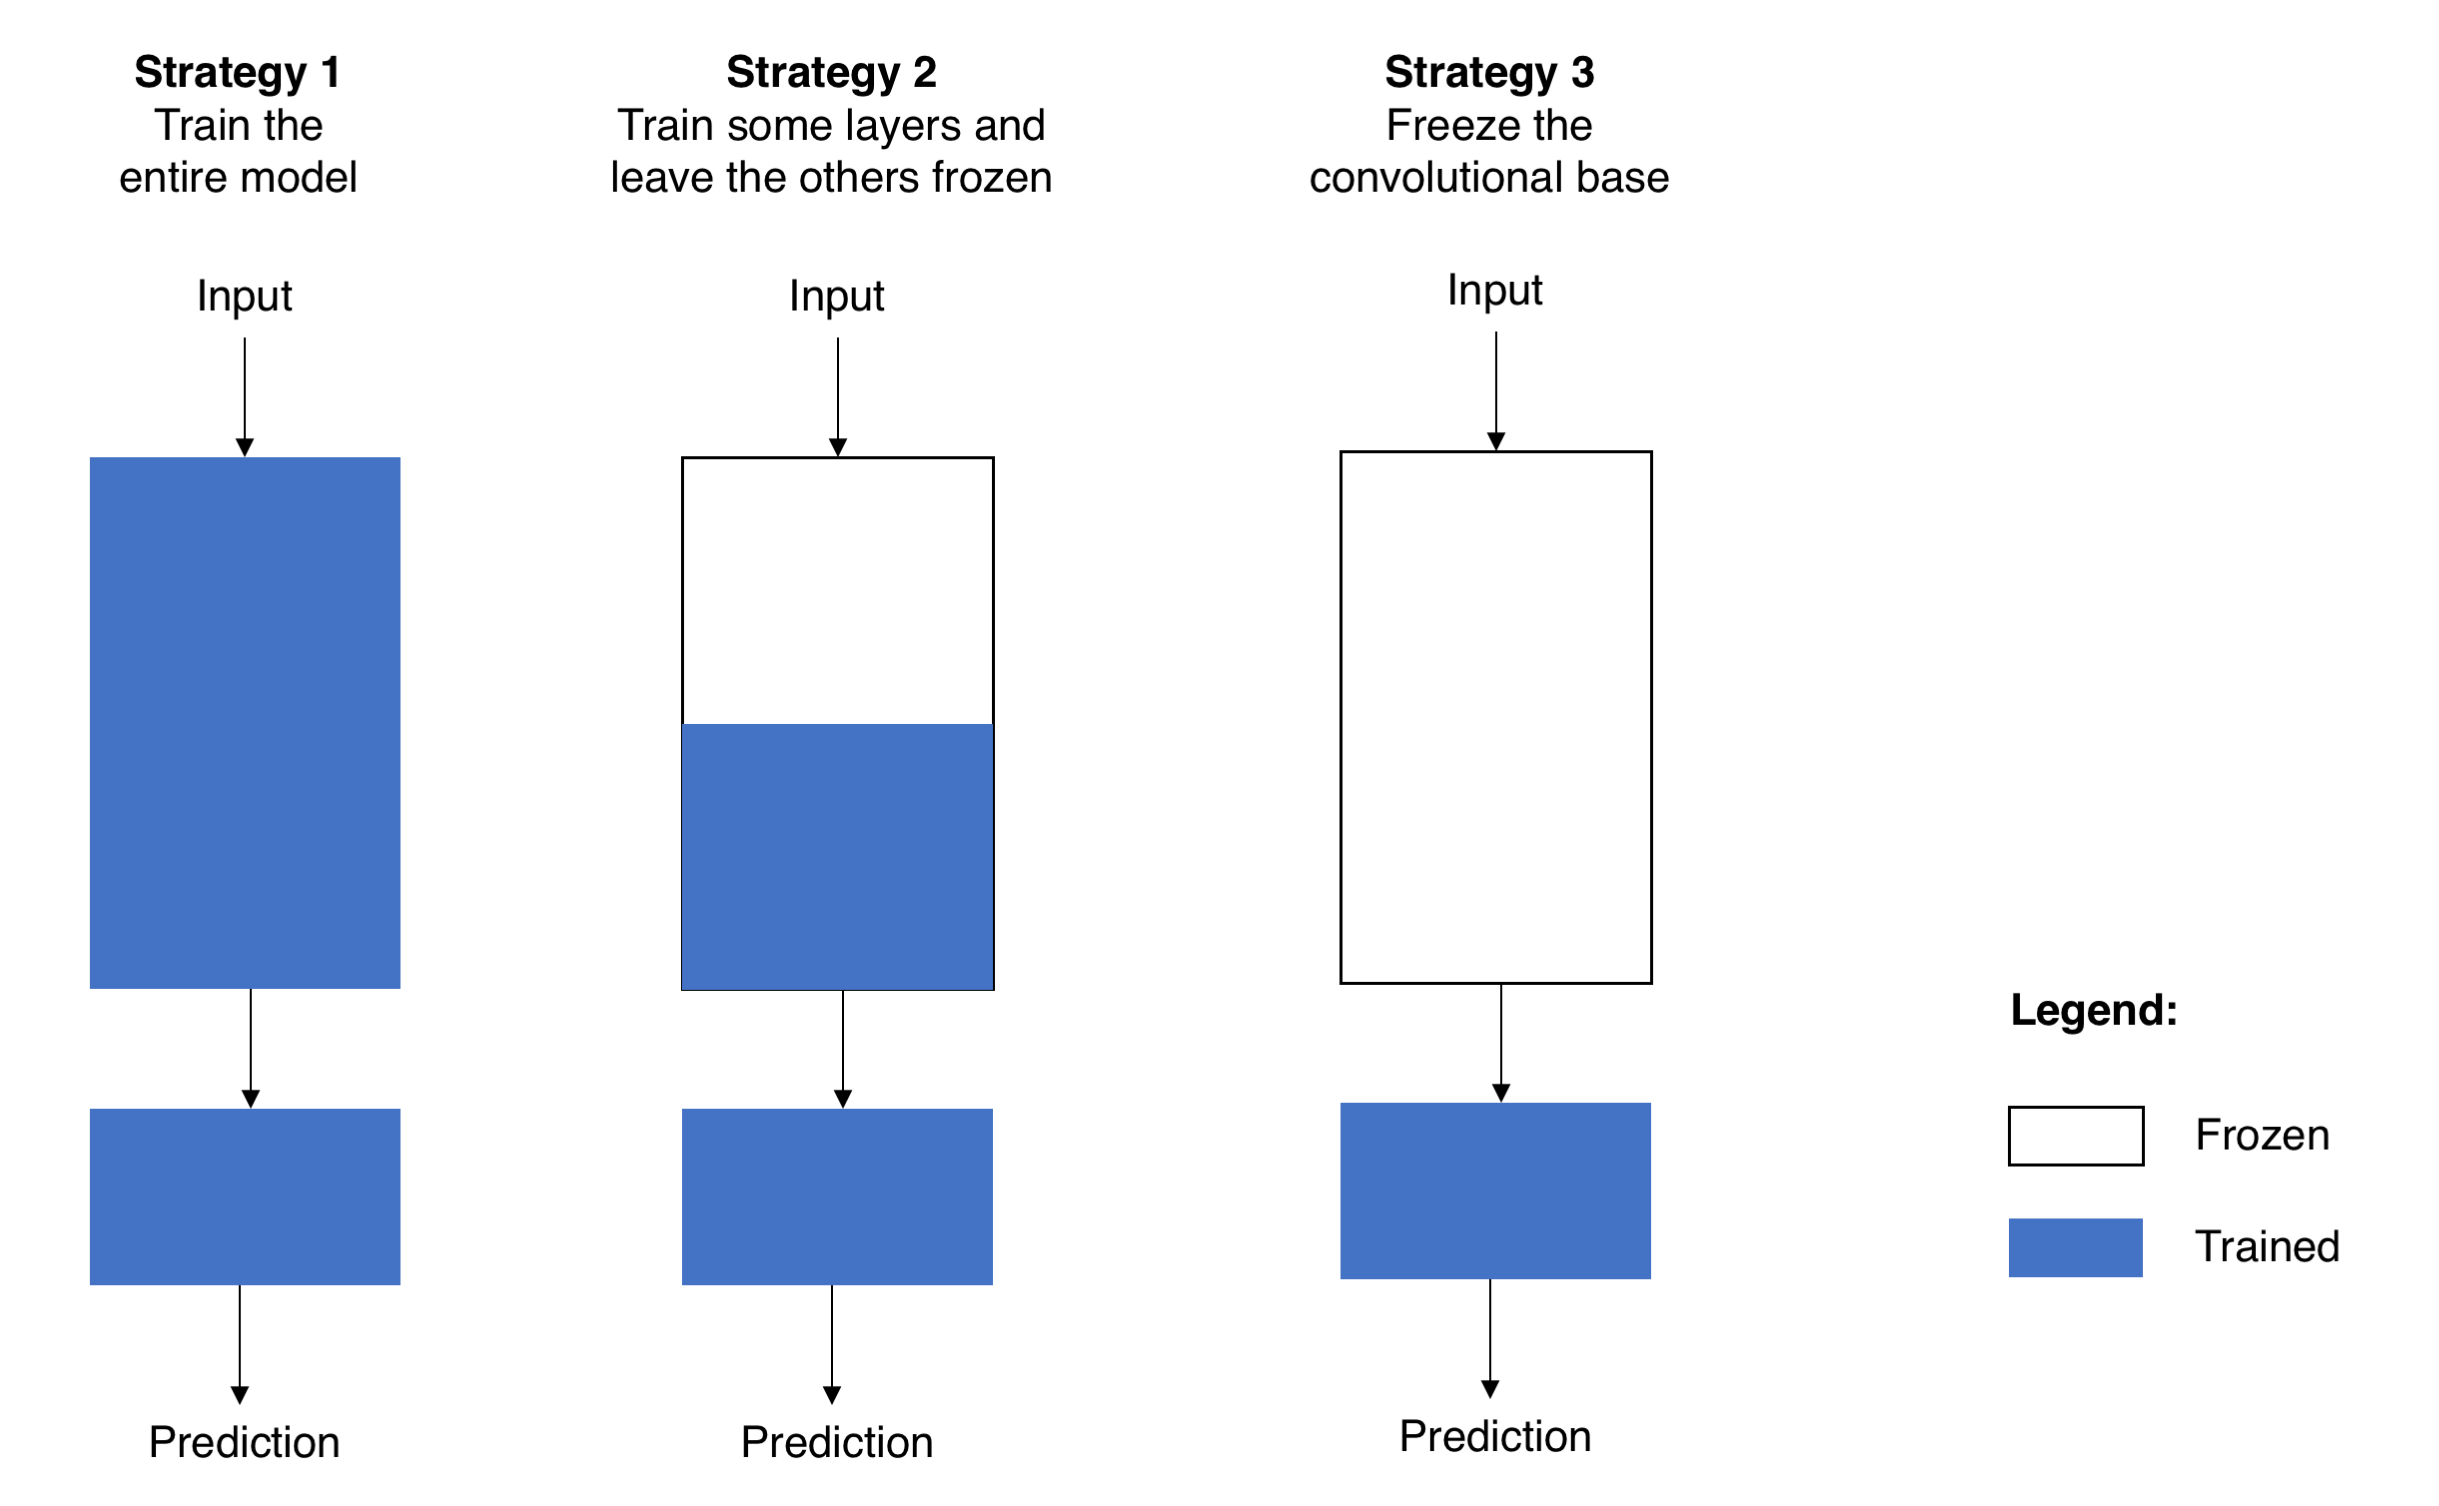
\includegraphics[scale=0.5, width=\linewidth]{figs/transfer_learning.png}
  \caption{Transfer learning fine tuning strategies \cite{marctransferlearning}}
  \label{fig:transferlearning}
\end{figure}

\subsection{Overfitting and underfitting}
While training, one must fine tune the model to both accurately make predictions from the training data while generalizing to new data. The bias and variance trade off is a well known problem in deep learning that represents a trade off between these two requirements. While the bias of a model is the error caused by the assumptions made to approximate the model to the true predictions, the variance of a model is the error from sensitivity to small fluctuations in the training set. We must find a good trade off between bias and variance so that the model doesn't underfit or overfit. \par
If the model underfits then it does not perform well even on the training data, and therefore has high bias and low variance. However, a common problem is to produce a model that performs well on the training data but that generalizes poorly to new data \cite{Grus}. In this case, we say that the model overfits and therefore has low bias but very high variance. In order to evaluate whether a model is underfitting or overfitting one should use state of the art metrics which help describe what is happening while training. \par  
Multiple solutions to the overfitting problem have been proposed and tested over the years. One common way of dealing with this problem are the regularization techniques, which are broadly described by some authors as any technique that allows the model to generalize better. For example, L1 and L2 regularization attempt to create less complex models \cite{Ng}, while techniques such as dropout "reduce complex co-adaptations between neurons" \cite{Hinton2012}. Other methods such as data augmentation can also minimize this problem.

REFERENCIAR FIGURA!!
\begin{figure}[ht]
  \centering
    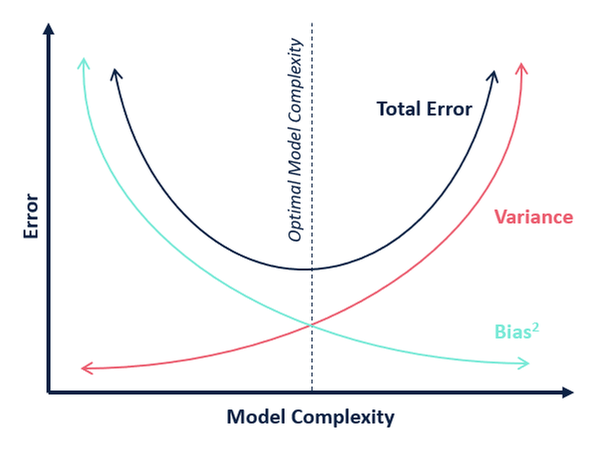
\includegraphics[width=0.5\linewidth]{figs/bias_variance_tradeoff.png}
  \caption{Influence of bias and variance on total error}
  \label{fig:biasvariancetradeoff}
\end{figure}

\subsubsection{Expanding the training data}
In deep learning, a model is highly dependent on its training dataset in order to achieve good performance.
A bad dataset can easily cause the network to overfit because it does not provide enough proper real world examples for the network to produce a good bias variance trade off. A good dataset has to represent the real world it tries to describe, be diverse, and most importantly, it needs to have a good number of examples.
There are several datasets available which are labelled for skin lesion diagnosis, but a lot of them are quite biased towards some specific class or lack large amounts of examples for a specific class. As such, when some real world variation is introduced the network fails to predict the class. \par
One way to improve the training dataset with low costs is through a concept called data augmentation. The main idea behind this concept is to expand the training data by applying operations that reflect real-world variation \cite{Nielsen2017a}, which in turn introduces diversification and size to the dataset. The simpler approach is to apply general transformations, such as translations, rotations or flips to existing samples to create new ones. Another more complex approach is to synthetically create new images based on some original dataset (generative models) through methods such as generative adversarial networks, a type of neural networks.

\subsection{Ensemble learning}
Neural networks are non linear methods, which means that they can learn complex non linear relatioships in the data. A downside of this flexibility is that they are sensitive to initial conditions, both in terms of the initial random weights and in terms of the statistical noise in the training dataset \cite{Brownlee}. As such, depending on it's initial conditions it may learn a very different version of the mapping function from inputs to outputs, which will directly impact the model's performance. This means that neural networks tend to have produce low bias and high variance. \par
One solution to this low bias high variance scenario is to use ensemble learning, which is a machine learning paradigm that combines multiple weak learners (models) that solve a particular problem in order to create a presumably better performing model. These are called weak learners because they often suffer from either high bias which usually happens to low complexity algorithms (e.g. linear regression) or high variance which is associated with high complexity algorithms (e.g. neural networks). \par
Ensemble learning is a studied field in that provides several methods to combine models. Those combinations are often based on 3 variations.
\subsubsection{Varying the choice of data}
The data used to train each member of the ensemble can be varied. 
The simplest approach would be to repeatedly sample the dataset with a random splits of the data into train and test sets. We can then train different models based on each of those samples and combine them together.  \par
An alternative would be to perform k-fold cross validation. For this procedure, k different models are trained on k different subsets of the training data. These models can then be saved and used as members of an ensemble. \par
Another approach is to perform bagging (short for bootstrap aggregating). Given a training dataset with size n, bagging generates m new training sets each of size k, by sampling from the original dataset uniformly with replacement (observations may be repeated). Then, m models are fitted using the m bootstrap samples and are combined by averaging the output for regression problems or voting for classification problems. \par

\subsubsection{Varying the choice of the models}
Training neural networks with different initial conditions will result in different models. This means that we can vary those initial conditions and combine the resulting models in order to reduce the variance. \par
A possible approach for this would be to use a different set of hyperparameters (e.g. learning rate or loss function used) or even a different set of model architectures. This will hopefully create an ensemble of models that is going to learn substantially different mapping functions between inputs and outputs, which will lower the correlation between predictions and in turn lower the resulting model variance.
An alternative to this method is to periodically save the best model during training, and then ensemble them. This method is called snapshot  ensemble. At the heart of snapshot ensembling is an optimization process which visits several local minima before converging to a final solution \cite{snapshot}. A variation for this method is to save models from a range of epochs, perhaps identified by reviewing learning curves \cite{horizontalvertical}. Stochastic gradient descent with warm restarts \cite{sgdr} is another variation in which the optimization procedure is changed during training (e.g. oscillating the learning rate) and the best models are saved on specific checkpoints.
\subsubsection{Varying the choice of the way that outcomes from ensemble members are combined}
A simple way to combine predictions is to calculate the average between prediction between different ensemble models. A variation of this is to.
A slightly more complex approach is to create a new model that learns how to combine the predictions of the different ensemble models, This approach is often called model stacking. \par
In more sophisticated methods such as boosting, ensemble members are added one at a time in order to correct the mistakes of prior models. Other approaches such as model weight averaging \cite{?} attempt to average the weights of neural networks with the same architecture, rather than their predictions. 
\subsection{Deploying deep learning models}
Deploying deep learning models requires careful orchestration of components such as a learner for generating models, a visualization tool to analyse and validate models and a serving framework which exposes models through an API. Usually, these components are hard coded together by custom scripts leading to high coupling and low cohesion. This poses problems for future expandability of such systems because simple changes can completely break the pipeline. Therefore, it is a priority to build these systems in a modular approach such that components are independent of each other. In addition, requirements such as easy-to-use configuration and tools, scalability and reliability should also play a big role when considering frameworks and tools to create a cohesive architecture for a production application. \par
Frameworks such as Tensorflow Extended\cite{Baylor2017} attempt to integrate the aforementioned components and requirements into one platform and standardize the whole process. Tensorflow has become a more production centered platform over the years, for example, by integrating Keras\cite{chollet2015keras} into it, which provides more easy to use high level concepts to train and test models. There are other options such as Theano\cite{Bastien} or pyTorch\cite{pytorch} but these are more focused around research environments. \par   
Training deep learning models usually requires high computational requirements, which is why nowadays most of these frameworks take advantage of GPUs through the CUDA platform. However, for small teams such computational power might be inaccessible or the cost of either time or money to setup such system might be too much. In such cases, it is better to take advantage of cloud services to train these models.  


\section{eHealth/mHealth for skin lesion diagnosis}
Online health, ehealth and mhealth applications represent a rapidly developing field of medicine that has the potential to become powerful tool in the diagnosis and management of skin diseases \cite{Jaworek-Korjakowska2018}. These applications aim to enhance clinical care, promote health, prevent diseases and most importantly provide medical support when it is not available at a particular location or time. Generally, the acceptance towards this type of systems in the medical community keeps growing, but is highly dependent on factors such as performance, accessibility and ease of use, which poses challenges for their global adoption \cite{?}. \par
Currently, several production ready skin lesion classification systems are  available for both skin professionals and patients wishing to self monitor their own skin. However, almost none of them has shown to be sufficiently accurate or reliable enough for a clinical environment. \par 

This subsection reviews the literature related with the development of dermatology applications for the self-surveillance of skin lesions. These applications offer the patient the ability to monitor their skin condition using images self-captured with a smartphone, while the capability for processing and displaying results is very variable. These efforts have been leveraged by the growing availability of smartphone attachments capable of turning these devices into compact dermatoscopes. Here, a chronological order is followed using a wide range of sources, including the contributions of Brewer et al. (2013), Kassianos et al. 2015 and Zaidan et al. (2018) that organized their surveys as a map of research concepts discussed in relevant literature. \par

Brewer et al. (2013) identified and categorized the variety of mobile apps available in dermatology, in May 2013, for both the general public and the dermatology providers. A total of 229 dermatology apps were identified in thirteen categories, the most important being the following: (i) general dermatology reference: 61 apps whose contents range from a short list of common skin conditions for the general public to a comprehensive reference guide for medical professionals; (ii) self-surveillance/diagnosis: 41 apps allowing users to document lesions, upload/receive dermatologist or algorithm-based feedback about malignancy potential of lesions, log personal treatment regimens and record symptoms to allergen exposures; (iii) sunscreen/UV recommendation: 19 apps provide sunscreen recommendations based on the skin type and the weather conditions; (iv) teledermatology: 8 apps allow for mobile consultation services; (v) dermoscopy: 2 apps were identified that require a proprietary dermoscope smartphone attachment.

Later, Kassianos et al. (2015) reviewed smartphone applications for the detection of melanoma targeted at the general community, patients and clinicians. The authors reported the existence of 39 dermatology-related applications available on the market, in July 2014, in a range of functionalities including information, education, classification, risk assessment and monitoring change. Over half of them provided information, advice or education about melanoma, ultraviolet radiation exposure prevention advice, and skin self-examination strategies, mainly using the ABCDE (A, Asymmetry; B, Border; C, Colour; D, Diameter; E, Evolving) method. Half of the apps helped users take and store images of their skin lesions either for review by a dermatologist or for self-monitoring to identify change, an important predictor of melanoma. A similar number of apps provide reminders to help users monitor their skin lesions. A few apps offered expert review of images. Four apps provided a risk assessment to patients about the probability that a lesion was malignant or benign, and one app calculated users’ future risk of melanoma. There was little evidence of clinical or research-based input into the design of these apps. Furthermore, none of the apps appeared to have been validated for diagnostic accuracy using established research methods.

More recently, Zaidan et al. (2018) reviewed the literature on smartphone applications for skin cancer diagnosis in the period from 2011 to 2016. A total of 89 articles were classified into four groups: development and design, analytical, evaluative and comparative, and review and survey studies. Out of the 89 articles, 43 focus on the development of various AI algorithms and applications for assisting in the prevention and early detection of malignant melanoma. A total of 20 articles involve analytical studies on the incidence of skin cancer, the classification of malignant cancer or benign cancer and methods for prevention and diagnosis. A total of 15 articles consist of studies that range from evaluation or comparison of mobile apps to the exploration of features designed for skin cancer detection. A total of 11 articles comprise reviews and surveys referring to actual applications or providing a general overview of the technology.

In the meantime, Jaworek-Korjakowska and Kleczek (2018) reported the existence of about 45 mobile applications related to mole diagnosis available on Apple’s App Store in March 2017. Most of them offered only educational information on melanoma, nearly half of them allowed the user to take photos of their moles and track changes over time using simple visual comparison, and only four applications performed melanoma risk assessment or lesion classification based on image analysis. These applications are DermaCompare (risk assessment through image matching), Lūbax (mole diagnosis through content-based image retrieval), MySkinApp (risk assessment) and SkinVision (risk assessment through fractal analysis). From these applications, two were certified by authorities, namely SkinVision received the European “CE” Marking and DermaCompare was approved by the U.S. Food and Drug Administration. \par

One of the most popular eHealth applications for this purpose is Metaoptima's Dermengine web application. Their Visual Search tool compares a user-submitted image with similar images in a database of thousands of pathology-labelled images gathered from  other dermatologists. Deep learning techniques are used to search for related images based on visual features such as colour, shape or patterns \cite{dermengine}. \par

Another popular app is the SkinVision which classifies lesions as either low, medium or high risk of skin cancer by using an risk assessment algorithm based on gray-scale images of lesions and their associated fractal maps. It achieves the overall sensitivity of 73\%, specificity of 83\%, and accuracy of 81\%. The positive and negative predictive values were 49\% and 83\%, respectively \cite{Jaworek-Korjakowska2018}. \par

\section{Skin lesion diagnosis}
Typically, in order to classify a skin lesion from dermoscopic images one must first segment the lesion, then extract relevant features from the segmented part of the image and finally classify the lesion into a specific class. \par

Skin lesions are often distinguishable from the surrounding area of the skin due to their color, intensity and texture. Lesion segmentation aims to separate that region from the rest of the image, in order to apply further processing it (e.g., identification of global morphological features specific to the lesion and segmentation of various local features at a later stage). This can become a challenging problem because  demoscopic images often come with various artifacts, like hairs, ruler marks, date markers, ink, bubbles etc. and in many cases there is a low-contrast between the bounded region and the surrounding area (due to the lighting conditions, skin tone variations and so on). Additionally, the lesion itself can have variations in color, texture, shape, size and location that make it difficult to contrast it with the background. Although the impact of these factors can be minimized with proper pre-processing.  \par

Therefore, both high and low level methods for performing lesion segmentation have been proposed over the years, including histogram thresholds, clustering, active contours, edge detection, graph theory and probabilistic modeling \cite{?}. \par

With the bounded region one can start feature extraction by identifying points of interest within that region. Such interest points are often attributes like color, texture, shape, structure, relative size and location of the lesion \cite{Barata2014}. As a result of several studies, multiple algorithms have been identified to help determine whether a given skin lesion is melanocytic/nonmelanocytic and benign/malignant, namely: 
\begin{itemize}
    \item Pattern analysis (Pehamberger and Steiner, 2016; Barzegari et al., 2005) identifies melanocytic lesions using local and global patterns. Local patterns include pigment system, dabs and globules, streaks, blue whitish shroud, relapse structures, hypopigmentation and vascular structures. Global patterns include reticular, globular, cobblestone, homogeneous, stardust, parallel, multi- component, lacunar and unspecific patterns.
    \item ABCD-rule (Nachbar et al., 1994) evaluates melanoma diagnosis using four criteria which include asymmetry, border irregularity, color and diameter. Each criteria is multiplied by a weight factor to establish a Total Dermoscopic Score (TDS) such as a lesion is considered benign for a TDS score lesser than 4.75, an intermediate TDS value of 4.75–5.45 it is regarded as possible melanoma and a score above 5.45 indicates probable melanoma.
    \item Menzies method (Robert, 2002) is based on a set of negative and positive features. Negative features include patterns that are point or axial asymmetric and presence of a solitary shading (gray, ebony, blue red, tan and dark brown). The nine positive features include blue white veil, multiple brown dots, pseudopods, radial streaming, depigmentation, peripheral ebony dots/globules, multiple hues, numerous blue/dark spots and expanded network. For a lesion to be classified as melanoma at least one positive feature must be found.
    \item 7-point checklist (Unlu, Akay and Erdem, 2014; Walter et al., 2013) assigns a score based on three major (atypical pigment network, blue-white veil and atypical vascular pattern) and four minor criteria (irregular streaks, irregular pigmentation, irregular dots/globules and regression structures). To score a lesion, the proximity of a major criterion is given 2 points and that of a minor model is given 1 point. The lesion is named as melanoma when the aggregate score is more prominent than or equivalent to 3.
    \item CASH algorithm (Henning et al., 2007) is designed as a simplified form of pattern analysis in which lesions are evaluated according to the color, architecture, symmetry and homogeneity.
\end{itemize}


Finally, the image features extracted can be fed to a classifier that should be able to distinguish, for instance, melanomas from benign lesions. Such classifier can be based on a multitude of algorithms such as artifitial neural networks or support vector machines. Figure \ref{fig:classificationalgorithms} illustrates the distribution of the most used algorithms for classifying features from skin lesions. \par

\begin{figure}[ht]
  \centering
    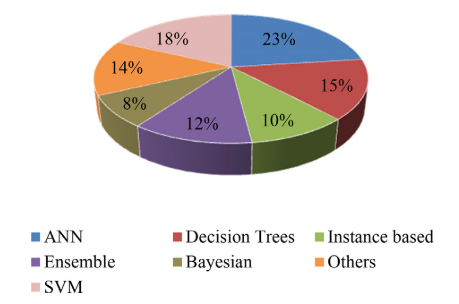
\includegraphics[width=0.5\linewidth]{figs/classificationalgorithms.png}
  \caption{Illustration of classification methods used by existing diagnostic methods \cite{Pathan2018}}
  \label{fig:classificationalgorithms}
\end{figure}

While these type of approaches provide a way of classifying skin lesions, they require domain knowledge, particularly, when performing segmentation and feature extraction. More recently end-to-end learning techniques have become prominent in fields such as medical imaging (and for skin lesion diagnosis in particular), meaning that no preliminary steps such as lesion segmentation or feature extraction are necessary. These techniques are often based on deep neural networks \cite{?}.

\section{Deep neural networks for medical imaging}
Deep learning refers to computational models composed of multiple processing layers capable of learning representations of data with multiple levels of abstraction \cite{Goodfellow-et-al-2016}. The initial impact of deep learning for medical imaging was revealed through a special issue published in 2016 at the IEEE Transactions on Medical Imaging \cite{Greenspan2016}. It explains the principles and methods of deep learning applied to medical image analysis. These structures can be found in approaches to medical imaging problems such as organ segmentation, lesion detection and tumor classification. \par
The main advantage of deep learning over other machine learning algorithms is that it removes the need for feature engineering, a process that requires knowledge of the problem domain, which can be a time consuming process as well as introduce human error.\par
Recently, deep neural networks appear as state-of-the-art solutions for medical imaging problems due to advancements in the field. These advancements include the research and development of new methods to prevent overfitting, the rise of computational power along with the use of graphical processing units, and finally the development of high level modules such as theano \cite{Bastien} that help train and test neural networks . 
\section{Skin lesion classification using deep learning}
One of the most important factors which determines the performance of a deep learning model is the dataset used to train it on \cite{?}. For general image recognition problems datasets such as ImageNet \cite{Deng2010} which contains over 14 Million samples with over 20000 classes are usually used and serve as a benchmark. However for skin lesion diagnosis systems, it is difficult and in many times impossible to compare the performance of published classification results since many authors use nonpublic datasets for training and testing \cite{Brinker2018}. The closest benchmark dataset available for this domain is the HAM10000 dataset \cite{ham10000} and consists of 10015 dermatoscopic images and contains classes such as Actinic keratoses and intraepithelial carcinoma / Bowen's disease (akiec), basal cell carcinoma (bcc), benign keratosis-like lesions (solar lentigines / seborrheic keratoses and lichen-planus like keratoses, bkl), dermatofibroma (df), melanoma (mel), melanocytic nevi (nv) and vascular lesions (angiomas, angiokeratomas, pyogenic granulomas and hemorrhage, vasc).\par
Nonetheless, organizations such as International Skin Imaging Collaboration (ISIC) provide an open source public access archive of skin images, which can be used for teaching or for the development and testing of automated skin lesion diagnosis systems \cite{isic2019}. They also place a challenge around their dataset every year in order to improve the performance of this classification systems as a whole. \par
\subsection{Transfer learning approaches}
Perhaps one of most popular approaches for skin cancer classification using deep learning, specifically, convolutional neural networks, was published in 2017 by Esteva et al.\cite{Esteva2017}, in which their classifier could diagnose keratinocyte and melanoma cancer. Their dataset combines biopsy-proven data from the ISIC archive, Edinburgh Dermofit Library, and the Stanford Hospital, totalling an astonishing 129450 samples (after going through data augmentation of random flips, rotations, crops) which remains one of the biggest efforts in data collection in the area.  The authors follow a transfer learning approach by leveraging the weights of the InceptionV3 network trained on ImageNet, on top of which they build their own classifier. Finally, they measured the network's performance by pitting it against 21 dermatologists on biopsy-proven samples and concluded that their classifier had comparable performance to that of those board-certified dermatologists.\par

Haenssle et al \cite{Haenssle2018} presented a very similar approach to Esteva et al \cite{}. They also fine tuned the Inceptionv3 model, but the analysis was limited to samples of melanoma versus benign nevi. However, they compared their approach with 58 dermatologists which is the largest number of dermatologists involved in a publication about skin lesion classification \cite{Brinker2018}. They achieved AUC ROC of 0.86, a slightly lower score than that of Esteva et al which stayed at O.94. \par 
More recently, 

Providing information and treatment options for a lesion, and detecting skin cancer with a reasonable sensitivity and specificity are the two main goals behind skin lesion classification on a clinical context. While the first goal is a multi-class problem (diagnosis out of range of classes), the second is a binary one ("biopsy" or "don't biopsy"). Contrarily to previous years where the presented challenges focused on binary problems (second goal), in the part 3 of the ISIC 2018 challenge participants were asked to develop a classifier to distinguish between 7 different types of skin cancer which focuses on the first goal. Those classes are:
\begin{itemize}
    \item Melanoma 
    \item Melanocytic nevus 
    \item Basal cell carcinoma 
    \item Actinic keratosis 
    \item Benign keratosis 
    \item Dermatofibroma 
    \item Vascular lesion
\end{itemize}

Participants were ranked based on the normalized multiclass accuracy (shown in equation \ref{eqs:bma} as it is closer to real evaluation of a dermatologist \cite{isic2018}, but other metrics such as accuracy, F1 score or AUC are computed for scientific completeness. An advantage of this metric is that algorithms can then be compared with physicians performance in skin lesion classification. \par 
\begin{equation} 
    B=\sum_{i}^{n} \frac{P_i}{n} \label{eqs:bma}    
\end{equation}
Where $P$ is the precision (or recall), which is given by equation \ref{eqs:precision}:
\begin{equation}
    P=\frac{TP}{TP+FP} \label{eqs:precision}    
\end{equation}

The top 3 submissions had balanced accuracies of about 88,5\%, 88,2\%, 87,1\% respectively and were all submitted by Aleksey Nozdryn-Plotnicki and Yolland which work at Metaoptima (the company behind Dermengine) \cite{isic2018top3}. To train those models they used the provided dataset, along with samples from ISIC archive and other proprietary data, that then they preprocessed by normalizing the samples with the Shades of Gray method \cite{shadesgray}. Additionally, they augmented the training data by performing random horizontal flips, random rotations, changes in brightness, saturation, and contrast. They used transfer learning from several pre trained models trained on ImageNet (such as InceptionV3 or ResNet) and then ensembled the best performing ones \cite{isic2018top3}. \par

Noteworthy are also the submissions by: 
\begin{itemize}
    \item Gessert et at. \cite{gessert2018} has a particularly interesting approach for inference (shown in Figure \ref{fig:gessert2018}), while performing effectively on task 3 with a balanced multiclass accuracy of 0.83 (fourth place). SENet154, ResNeXt101, Densenet201, Densenet161, Densenet169, SE-Resnet101 and PolyNet are the pre-trained models used for ensembling. For each architecture 6 models are trained, 5 by performing 5-fold cross validation and 1 by training it with the whole dataset (without validation set). Evaluation is performed by cropping 36 patches from each test sample and feeding those patches to each model. Then, for the models that do not have a validation set, the softmax probabilities are averaged across all 36 patches. and for models that were cross validated, predictions are combined using an Support Vector Machine. Finally, both results are combined by averaging the softmax probabilities.
    \begin{figure}[ht]
        \centering
        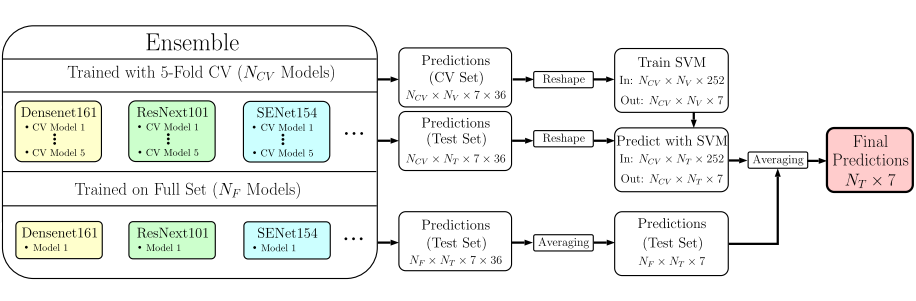
\includegraphics[width=\linewidth]{figs/gessert2018.png}
        \caption{Gessert et al's evaluation strategy for the generation of the final predictions. \cite{gessert2018}}
        \label{fig:gessert2018}
    \end{figure}
    \item Ashraful Alam Milton \cite{Milton2018} who also followed an approach based on transfer learning from models of PNASNet-5-Large, InceptionResNetV2, SENet154, InceptionV4 trained on ImageNet, who interestingly noted that in the first few epochs the gradient is very erratic and thus refrained from fine-tuning weights during the first 2 epochs to avoid updating weights towards the wrong direction, in the end achieving a score of 0.76 on the validation set;
    \item Bissoto, Perez, Ribeiro, et al. \cite{Bissoto2018} (who won 3rd place in the 2017 edition) which transfered knowledge from models of InceptionV4, ResNet-152, and DenseNet-161 trained on ImageNet, by training with online data augmentation (e.g., random crops, flips, rotations, shears, color transformations), SGD with the learning rate being decreased by a factor of 10 whenever validation loss didn’t improve for 10 epochs, eventually building an average of 15 models trained only with the challenge data that attained a score of 0.803.
\end{itemize}

Tschandl et al \cite{humanvsisic2018} compared the diagnostic accuracy of 139 machine-learning algorithms from ISIC 2018 with 511 human readers, with the large majority being board-certified dermatologists (55.4\%), 23.1\% being dermatology residents and 16.2\% being general practitioners. Machine learning algorithms outperformed human readers on the large majority of measures, for instance, in sets of 30 randomly selected lesions, the best machine-learning algorithms achieved a mean of 7.94 more correct diagnoses than the average human reader, and a mean of 6.65 more correct diagnoses than expert readers. However, authors advocated that higher accuracy does not necessarily mean better clinical performance or patient management For instance, these algorithms were trained to optimise the mean sensitivity across all classes, and did not consider that it is more detrimental to mistake a malignant for a benign lesion than vice versa. They also found that the difference between human experts and the top three algorithms was significantly lower for images in the test set that were collected from sources not included in the training set (out of distribution samples), and noted this might be a possible limitation of these algorithms which should be addressed in future research. Other authors such as Han et al, also noted this same limitation in their study \cite{Han2018}. \par 

As a response to this unresearched matter, ISIC 2019's challenge asked participants to classify dermoscopic images among nine different diagnostic categories, with 8 known classes (i.e. Melanoma, Melanocytic nevus, Basal cell carcinoma, Actinic keratosis, Benign keratosis, Dermatofibroma, Vascular lesion, Squamous cell carcinoma) and one "unknown" class which conceptually means none of the other classes. Similarly to the 2018's version participants could use their own data to improve the network's performance and were ranked based on a balanced multiclass accuracy \cite{isic2019}. \par

The best submission was done by Geesert et al. (which was the team that achieved fourth place at ISIC 2018 Task 3) scoring 0.636 balanced multiclass accuracy \cite{isic2019first}. 
In adition to the challenge's dataset, 995 dermoscopic images from the 7-point dataset \cite{?} and 1339 images from an in-house dataset were used for training. More specifically, the in-house dataset also contains additional images that were used for the unknown class  
Before training images need to be preprocessed which is performed by cropping the images, performing image binarization, then applying the shades of gray color constancy method \cite{shadesgray} and finally resizing the images (longer side to 600 pixels while keeping the aspect ratio). 
Data augmentation is also applied before training by randomly changing brightness, contrast, rotation, scale, shear, flip and finally by adding  Cutout \cite{cutout} holes.  
The authors opted to use two different input strategies, which leads to having different models each with different configurations. The first strategy takes a random crop from the preprocessed image, but the second strategy randomly resizes and scales the image when taking a crop. 
Like the previous attempts they use a transfer learning approach relying on ImageNet pre-trained models, namely, multiple versions of EfficientNets and a SENet154 which was allegedly added for architecture variability. All models were trained for 100 epochs using the Adam optimizer \cite{adam} and a weighted cross-entropy loss function to deal with class unbalance.
Predictions for each model are made based on which input strategy was used. The final prediction is made using an ensemble of a subset which contained all the best performing models. \par

At second place, Zhou et al's \cite{isic2019second} achieved a balanced multiclass accuracy of 0.607. Unlike, Gessert et al. no additional data was used for training and testing. Images are resized but maintain the aspect ratio (with the shorter edge having 600 pixels) and the shades of gray color constancy method \cite{shadesgray} is performed. Images are augmented using random cropping, scaling, rotations and color transformations. Like most submissions, they used a transfer learning approach by fine tuning Densenet121, se-resnext50, se-resnext101, EfficientnetB2, EfficientnetB3 and EfficientnetB4 which were all pre trained on ImageNet. 5-fold cross validation was performed with a 80-20 split, and models were trained for 90 epochs with the Adam optimizer \cite{adam} with learning rate 5e-5 but decreased by a factor of 2 after 10 epochs. To address the unbalanced class distribution, the authors trained all networks with a weighted loss function where weights are determined using the inverse frequency of classes in the training data. For the ensemble, multiple subsets of models were tested in order to optimize the normalized multiclass accuracy values, but for the final submission EfficienetB3, EfficienetB4 and Seresnext101 were used. During inference, for each test image, N (either 16 or 25) ordered same-sized patches are fed into each network and the final prediction is obtained by averaging the prediction probabilities. Finally, the unknown samples are handled by simply classifying the images whose top-1 probability are less than 0.35 as unknown.\par

At third place Pollastri et al. \cite{isic2019third} uses a more complex approach for dealing with the unknown class. Two models were created in their approach called baseline model A and B with the following procedure:
\begin{itemize}
    \item Preprocessing is done by padding samples with reflection in order to rescale them them to a square size of 512x512 pixels. Pixel intensities are normalized to have 0 mean and 1 standard deviation.
    \item Training is performed using a cross entropy loss function which is weighted according to the inverse prior probability of each class, which according to the authors helps with the data unbalance problem in the sense that avoids situations where the network performs a maximum likelihood optimization, where it becomes biased towards the most probable class. 
    \item For baseline model A, DenseNet201, ResNet152 and SeResNext101 were the pre trained models used, while for baseline model B, SeResNext-50, SeResNext-101 and the SeNet-154 were the preferred models.
    \item Both baseline models use online data augmentation. Baseline model A uses operations such as rotations, flips, Gaussian blur, adding Poisson noise, gamma contrast changes, Cutout augmentations \cite{cutout} (0 to 3 holes with different sizes), hue/saturation changes. These are then combined in different ways to form an ensemble composed of multiple pre-trained models with different architectures and different data augmentation methods. In contrast, baseline model B uses similar operations but the augmentation configuration is the same across all models.
    \item Inference in baseline model A is performed by ensembling the results from 21 models (each trained with different pre-trained models and augmentations) for a given sample, but test samples also go through the same augmentations as the ones performed during training. For baseline model B a snapshot ensemble technique \cite{snapshot} was used. 
    \item Their proposition to determine the unknown class is to use the Out of Distribution Detector by \cite{Vyas2018}. 8 CNNs (Densenet-201) are trained to classify if a given sample is part of the training dataset or if it is an out of distribution sample. Each model employs 7 classes as inside distribution data, and 1 class as out of distribution, but the left out class is alternated in each of them. Inference is performed in a voting scheme where each network votes whether a given sample is part of training set or not.
\end{itemize}
Baseline model A and B are then combined together for the final submission which scored a balanced multiclass accuracy of 0.593. \par 

Hsin-Wei Wang approach \cite{Wang} is particularly note worthy because the materials for replicating his submission are available on Github. His method achieved a balanced multi-class accuracy of 0.505, a substantially worse performance than the best approaches mainly due to the poor results of the out of distribution detector on the unknown class. These are the main aspects of his methodology: 
\begin{itemize}
    \item In addition to the provided challenge dataset, 134 samples were obtained from the ISIC archive and the 7-point dataset to be used as unknown samples during testing. 
    \item Images were resized to fit the network's input size and normalized by per channel mean and standard deviation, which were calculated over the entire training set. 
    \item Similarly to the best approaches an ensemble of models was used which was created by taking the average of softmax probabilities made by three models (pre trained with the ImageNet dataset), the DenseNet201, Xception and ResNeXt50 . During training, first all layers are frozen first for weight initialization of the classifier for 3 epochs, then all the layers are unfrozen and fine tuned during 100 epochs with the Adam optimizer \cite{adam} and with a learning rate of 10e-5 which is reduced by a factor of 10 if the validation loss has stopped improving for 8 epochs. 
    \item In order to prevent overfitting, online data augmentation is performed with random crops, random flips, random rotations, random changes on brightness, and finally random changes on saturation.  
    \item Finally, for the unknown class the author took advantage of an already implemented method called ODIN (Out-of-Distribution detector for Neural networks) \cite{odin} which depending on 3 parameters (temperature scaling, perturbation magnitude and threshold) and based on the softmax predictions, could determine if a given sample is part of the training classes or not (in/out of distribution), 
\end{itemize}
\subsection{End to end learning approaches}
The most common approach to skin lesion classification is through transfer learning. However, end to end learning can make sense in specific contexts. For instance, when data and computational resources is not scarce. \par 
In 2019, Ly et al. \cite{Ly2019}, trained multiple models from scratch with the intention of deploying such models for offline usage in smartphones. They justified this decision by arguing that using pre trained models with large neural network architectures requires a lot more parameters than models trained from scratch. Their best model attained 86\% accuracy, significantly better than other transfer learning approaches, while being much more compact (29M). However, they used a huge dataset titled "PHDB" which was composed of multiple other datasets and contained 80,192 labeled images, which explains the high performance.


%\include{chapter3}
%\include{chapter4}



% End of Thesis text ---------------------------------------------------------
% Including files is advised:


%Appendix

\backmatter


%Print all used references

\begingroup
\renewcommand{\bibfont}{\footnotesize}

%Redefine References name
\defbibheading{bibliography}[Referências]{
	\chapter{#1}
}
\SingleSpacing
\setlength\bibitemsep{8pt}
\printbibliography[heading=bibliography]
\endgroup


%Load appendix
%\include{appendix-a}


\end{document}
